\section{Problem Definition}
\begin{figure}
    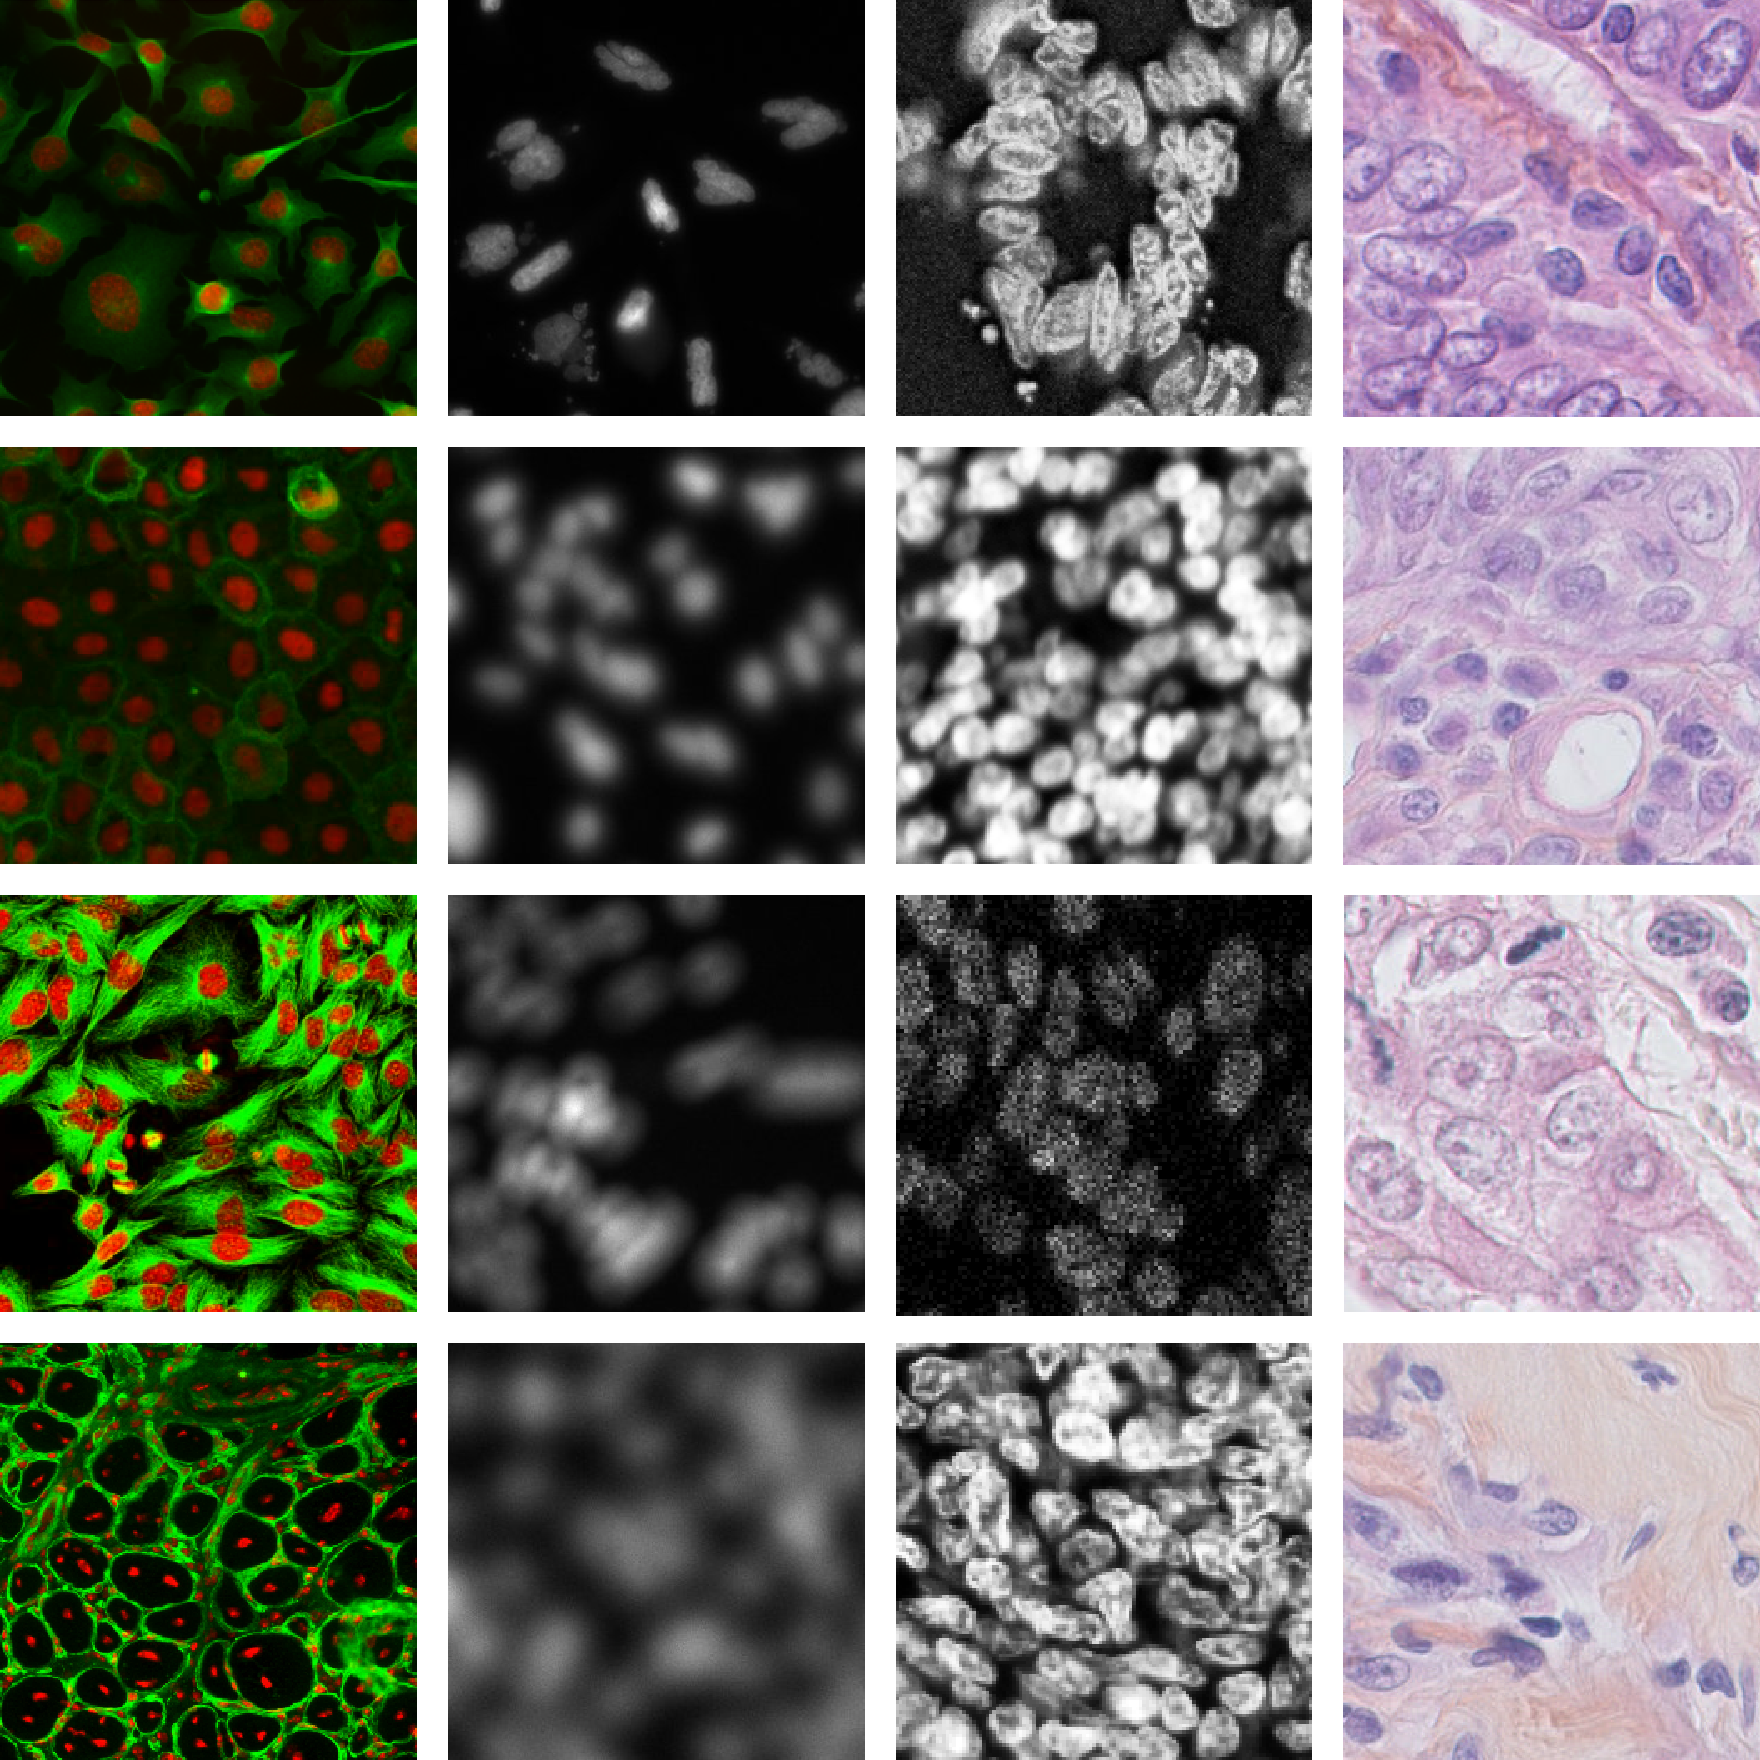
\includegraphics[width=\linewidth]{figs/Modality_Samples_4x4.pdf}
    \caption{\textbf{Illustating variability across microscopy imaging modalities and types.} First column describes images collected from Cellpose Gen. data~\cite{stringer2021cellpose}, second column represents various images of Human U20S cells with Hoechst and phalloidin stains from BBBC006~\cite{ljosa2012annotated}, the third column illustrates images from  Tissuenet~\cite{greenwald2022whole}, and the forth column shows results obtained using H \& stain from TNBC~\cite{naylor2018segmentation}.}
    \label{fig:modality}
\end{figure}


We are interested in improving tasks such as cellular activity monitoring. Various microscopes can be employed to produce videos of time-sequence observations in 2D and 3D volumes. For example, light-sheet, fluorescent, or confocal microscopy, each requiring tracking the cells in the volume they occupy. In \Cref{fig:modality}, we show different imaging data obtained using different platforms and on different tissue types. Given the variability among cells, which can differ in size and shape as well as in imaging modalities, it is evident that no single method can be generalized for all types of cell monitoring. According to \cite{bragantini2024ultrack}, this issue largely stems from the low-quality segmentation algorithms that introduce noise into the predictions, making it difficult to accurately link cells for lineage tracking. We align with this perspective and propose to address the test-time adaptation problem in cell instance segmentation to improve cell tracking in this manuscript.
 
\section{Methods}

\subsection{Overview}
Our hypothesis is that performing test time adaptation on cell segmentation will improve cell tracking performance since the associations are based on simple metrics such as IoU and Euclidean distance of the centroids~\cite{bragantini2024ultrack}. In our approach, we assume to have a pre-trained network available that was trained on a source dataset. Given that Cellpose~\cite{stringer2021cellpose} remains one of the leading algorithms for cell instance segmentation, we have selected it as our baseline algorithm and will build our TTA framework on top of it. In the sections that follow, we will provide an overview of the fundamentals of Cellpose~\cite{stringer2021cellpose}, discuss TTA, and outline our proposed framework.



\subsection{Cell Segmentation}

To test our hypothesis, we use one of the state-of-the-art cell instance segmentation algorithms as our segmentation framework Cellpose~\cite{stringer2021cellpose}. It is pretrained on diverse datasets and has good generalization capability. However, it is not pretrained on all imaging modalities or cell types, rendering it less useful in out-of-distribution datasets. We propose to utilize their pretrained model and perform test-time adaptation. 

Here, we describe the inner workings of Cellpose~\cite{stringer2021cellpose}: given an image $I$, the model uses a network $f$ to generate a dense, pixel-wise feature map $\bm{Z} = f(I)$, where $ \bm{Z} = [Z_1, Z_2, Z_3] \in \mathbb{R}^{h \times w \times 3}$. For some pixel $i$, we denote the feature $\mathbf{z} = [z_1, z_2, z_3] \in \bm{Z}$. Here, $\bm{z} \doteq (z_1, z_2)$ represents the gradient pointing towards the center of the cell structure to which pixel $i$ belongs. Together, $(Z_1,Z_2)$ form a \emph{gradient flow}. The component $z \doteq z_3$ represents the unnormalized score indicating the probability that pixel $i$ is part of a cell structure. It is worth noting that with this notation, the feature $\mathbf{z}$ can be written as $\mathbf{z} = [\bm{z}, z]$. The network $f$ is trained in a supervised manner with pixel-wise instance segmentation loss defined as follows:
\begin{equation}
 \mathcal{L}_i^{IS} = (z_1 - \mathtt{g_x})^2 + (z_2 - \mathtt{g_y})^2 + \nu H(\mathtt{m},\sigma(z))  \; ,
\end{equation}
where, for pixel $i$,  $(\mathtt{g_x}, \mathtt{g_y})$ represents the ground-truth gradient label with unit $\ell_2$-norm, $\mathtt{m} \in \{0, 1\}$ is the binary mask label indicating absence or presence of a cell structure, and $\sigma(z) \doteq 1/(1+\exp(-z))$ is the sigmoid function. The term $H$ represents the binary cross-entropy, and $\nu$ is a hyperparameter set to $0.04$. The contributions to the pixel-wise loss are aggregated into a final loss, $\mathcal{L}^{IS} = \sum \mathcal{L}_i^{IS}$ for the image $I$.


Given the feature $\bm{Z}$, the cell instance segmentation head $g$ produces the mask $Y = g(\bm{Z})$. For each pixel $i$, the predicted label $y$ takes the value from the set $\{0, 1, \cdots, N \}$, where $N$ represents the total number of segmented cell instances. Pixels that belong to the same cell instance share the same label, and $y=0$ indicates the absence of a cell instance. 


\subsection{Test-Time Adaptation Loss Computation}

At test-time, we follow two TTA constraints: \\
\indent (i) no source data available and \\
\indent (ii) no target labels available \\
In this setting, we want to perform the adaptation in a fully unsupervised manner. Once we have a pre-trained Cellpose~\cite{stringer2021cellpose} model available, we will utilize its predictions on the target data to perform the adaptation. 

\subsubsection{Self-Entropy}\label{sec:tta-se}
One of our first objectives is to calculate the Shannon entropy~\cite{shannon1948mathematical} of the mask probability predictions. Shannon entropy~\cite{shannon1948mathematical} allows us to quantify the model uncertainty in the model predictions. As it refers to the uncertainty of the model, we could also utilize this information as a metric to decide which predictions are confident predictions. It is especially crucial as data distributions can change during inference. As our mask predictions are given by $\sigma(z)$, our Shannon entropy~\cite{shannon1948mathematical} becomes the following:

\begin{equation}
    \mathcal{L}_i^{SE} = -\sigma(z) \log \sigma(z) \; ,
\end{equation}

However, since our mask predictions refer to a binary crossentropy task and do not possess a probability distribution over $k$ classes, we redefine the entropy as the following:
\begin{equation}
    \mathcal{L}_i^{SE} = -(\sigma(z) \log \sigma(z) + (1-\sigma(z)) \log (1-\sigma(z))) \; ,
\end{equation}

Now that we calculated $\mathcal{L}^{SE}$ for the binary mask predictions, we can use this information to collect more confident prediction. We choose a threshold $\delta$ that describes if the $\mathcal{L}_i^{SE}$ is lower than the threshold, then the predictions are confident enough. It is given by $\hat{\bm{z}} = \bm{z}[\mathcal{L}^{SE}<\delta]$. Further, once the indices are collected, we choose a probability threshold $p$ that determines if the original predictions have large enough probability to be considered a valid prediction which is given by $\hat{\bm{z}} = \hat{\bm{z}}[\sigma(z)>p]$. Now, we have a refined set of indices which will be useful in the next section. 

\subsubsection{Contrastive Flow Loss} \label{sec:tta-cfl}
The proposed framework utilizes a contrastive prediction task to enhance the gradient flow features of target pixels.  CellTranspose~\cite{keaton2023celltranspose} was the first to introduce a contrastive objective for the gradient flow alignment task, and we adopt their formulation in this paper. However, unlike their supervised framework, our approach employs contrastive learning in a self-supervised manner. \\

In our method, we define a positive sample using a refined binary mask from $\hat{z}$, represented as $\mathbb{I}[\hat{z}>p]$, which we denote as $\hat{z_+}$ (where $\hat{z} > p$). We then identify the gradient flow features $\hat{\bm{z}}_+$ that are closest to the prediction $\hat{\bm{z}} = (z_1, z_2)$ using a similarity metric. Specifically, we utilize cosine similarity, defined as $s(\bm{u}, \bm{v}) \doteq \frac{\bm{u}^T \bm{v}}{\| \bm{u} \| \| \bm{v} \|}$, with $\| \cdot \|$ denoting the $l_2$-norm. Next, we compile a set of negative samples $\mathcal{N}_i = \{\hat{\bm{z}}_- \; | \; s(\hat{\bm{z}}_+, \hat{\bm{z}}_-) < \theta, \hat{z}_- > p\}$, where $\theta$ is a hyperparameter threshold that we select. After gathering the positive and negative samples, we apply our contrastive objective for pixel $i$, aiming to pull the positive pairs $(\hat{\bm{z}}, \hat{\bm{z}_+})$ closer together while pushing the negative pairs $(\hat{\bm{z}}, \hat{\bm{z}}_-)$ apart. \\

Furthermore, \cite{wang2021understanding} recommends effective hard-mining strategies for learning with a contrastive objective. By implementing hard-mining for negative samples, we can reduce the need for a large number of negative samples while enhancing convergence speed. Since our objective adapts at test time, rapid convergence greatly benefits the algorithm. Therefore, similar to \cite{keaton2023celltranspose}, we adopt a hard-mining sampling strategy for negative samples. Essentially, $\mathcal{N}_i$ consists of pixels that are in close proximity to the positive samples. For more details, please refer to \cite{keaton2023celltranspose}.\\

Given a batch of target image patches, each patch is paired with another patch from the same batch. We then compute the contrastive flow loss aggregating all the components coming from all the valid pixels, i.e.,  $\hat{z}_- > p$. 
Now the loss function becomes the following:

\begin{equation}
    \small
    \mathcal{L}_i^{CF} = - \log \frac{\exp( s (\hat{\bm{ z}}, \hat{\bm{ z}}_+)/\tau )}{ \exp( s (\hat{\bm{ z}}, \hat{\bm{ z}}_+)/\tau ) + \sum_{\hat{\bm{ z}}_- \in \mathcal{N}_i} \exp( s (\hat{\bm{ z}}, \hat{\bm{ z}}_-)/\tau ) }\\
    \label{eq-contrastive-flow-loss}
  \end{equation}
where $\tau$ refers to a temperature parameter we choose. 

\subsubsection{Adaptation Loss}
In \cref{sec:tta-se}, we calculate self-entropy for the binary mask predictions and in \Cref{sec:tta-cfl}, we calculate a contrastive object to enhance the gradient flow estimations. We combine this two losses for the model update at test time as shown below:
\begin{equation}
    \small
    \mathcal{L}^{TTA} = \lambda_1\frac{1}{| \mathcal{M}_1 |} \sum_{\mathcal{M}_{1}} \mathcal{L}^{SE}_i + \lambda_2\frac{1}{| \mathcal{M}_2 |} \sum_{\mathcal{M}_2} \mathcal{L}^{CF}_i \; .
    \label{eq-tta-loss}
  \end{equation}
Where, total pixel belonging to the target patch, we define it by $\mathcal{M}_1$, and the valid pixels we define that set by $\mathcal{M}_2$. $\lambda_1$ and $\lambda_2$ are the weight parameters for the loss. This combination of losses is used to perform the adaptation. In the next section, we will discuss what parameters we want to update during TTA. 

\subsection{Test-Time Adaptation Parameter Updates}
Studies have shown that the major cause of performance degradation in convolution-based networks is the shift in batch-normalization statistics during inference~\cite{wang2020tent,niu2022efficient,zaveri2025improving,li2016revisiting,mirza2022norm,pan2018two,schneider2020improving}. We take advantage of these findings and propose to only update the batch-normalization parameters. They are calculated by the following equations:

\begin{equation}\small
    \centering
    \label{eq:bn}
        \begin{aligned}  
        BN(x) = \gamma \frac{x - E(x)}{\sqrt{Var(x)}} +  \beta ,
        \end{aligned}
\end{equation}
\begin{equation}\small
    \centering
    \label{eq:bn_running}
        \begin{aligned}  
            \overline{\mu}_t = (1-\alpha)  \overline{\mu}_{t-1} +  \alpha  {\mu}_t ,\\
            \overline{\sigma}_{t}^2 = (1-\alpha) \overline{\sigma}_{t-1}^2 +  \alpha {\sigma}_{t}^2 ,
        \end{aligned}
\end{equation}

where $x$ is the input feature, $E(x)$ and $Var(x)$ are the expected value and variance of $x$. $\gamma$ and $\beta$ are learnable parameters for scaling and shifting. The BN layers keep track of the running mean and variance through Equation \ref{eq:bn_running}, where ${\mu}_t$ and ${\sigma}_{t}$ are current expected value and variance respectively, and $\overline{\mu}_t$ and $\overline{\sigma}_{t}$ are used for $E(x)$ and $Var(x)$, respectively. $\alpha$ is the momentum parameter. We propose to estimate the learnable parameters $\gamma$ and $\beta$ during testing that requires a backward pass. Additionally, we also dynamically updates the BN statistics $E(x)$ and $Var(x)$ during testing according to the following strategy:
\begin{equation}
  \centering
  \label{eq:bn_update}
      \begin{aligned}  
          \overline{\mu}_{I,t} &= (1-\lambda{_{BN}}) \overline{\mu} +  \lambda{_{BN}} \mu_{I,t} \; ,\\
          \overline{\sigma}_{I,t}^2 &= (1-\lambda{_{BN}}) \overline{\sigma}^2 +  \lambda{_{BN}} \sigma_{I,t}^2 \; ,
      \end{aligned}
\end{equation}
where $\overline{\mu}$ and $\overline{\sigma}^2$ are the final running mean and variance of the model trained on the source data, respectively, and $\mu_{I,t}$, and $\sigma_{I,t}^2$ are mean and variance calculated from the instance at time $t$, respectively. $\overline{\mu}_{I,t}$ and $\overline{\sigma}_{I,t}^2$ are updated based on the current instance and used for feature normalization at time $t$. $ \lambda{_{BN}}$ is set to 0.1. 
